%%%%%%%%%%%%%%%%%%%%%%%%%%%%%%%%%%%%%%%%%%%%%%%%%%%%%%%%%%%%%%%%%%%%%%%%%%%%%%%
% template.tex - version 0.9.1.1 (5/26/2011)
%
% This is a template file for the osudiss-2 class. See
% osudiss-2.pdf for documentation, and the GS material 
% for the requirements.
%
% Copy the following osudiss-2 files your latex path (or just the folder containing this file):
% osudiss-2.cls (v0.9.1)
% sa-draftwater.sty
%
% Then, to compile this file:
% latex template
% bibtex template
% latex template
% latex template
%
% (You can also use pdflatex if you prefer.)
%
%%%%%%%%%%%%%%%%%%%%%%%%%%%%%%%%%%%%%%%%%%%%%%%%%%%%%%%%%%%%%%%%%%%%%%%%%%%%%%%
\documentclass[11pt, draft, onehalf, phd]{osudiss-2} 
% The `11pt' option is unnecessary since it is the default

% `onehalf' sets the line spacing to one-and-a-half spacing instead of
% double spacing.

% The `phd' option is unnecessary since it is the default

% Remove `draft' option for final draft

%%%%%%%%%%%%%%%%%%%%%%%%% Packages %%%%%%%%%%%%%%%%%%%%%%%%%
% Load your favorite packages here
\usepackage{graphicx} % for importing images in figures - you definitely want this!
\usepackage{lipsum} % for fake latin text---you probably don't want this

% For instance... see osudiss-2.pdf for some suggestions, if you don't
% have a clue
\usepackage{bm} % for bold math---useful
\usepackage{booktabs} % for more professional tables

%hyperref packages and options
\usepackage{bookmark} % helps booksmarks look better in PDF
%hypersetup option 'breaklinks' is reguired for line wrapping in the table of contents during latex compilation, and can be removed if you use pdflatex
\hypersetup{colorlinks=true,linkcolor=blue, breaklinks} %internal links in blue, citations in green
%\hypersetup{colorlinks=true,linkcolor=black, citecolor=black, breaklinks} %all links in black
\usepackage[all]{hypcap}

%Use of natbib is STRONGLY recommended to sort and compress your references within each citation
%With these options, natbib will convert i.e. [5,3,9,4] to [3-5, 9]
\usepackage[sort&compress]{natbib}

%required to have latex automatically generate subfigures (i.e. (a), (b) etc)
\usepackage{subfig}

%load glossaries packages
\usepackage[acronym, section=chapter]{glossaries}
%\usepackage[xindy,acronym, section=chapter]{glossaries} - recommended if supported by your OS
\makeglossaries %required to actually make a glossary
%A list of common acronyms
%Only those used will be displayed, so you can just add to this list
\newacronym{AFM}{AFM}{atomic force microscopy}
\newacronym{BCS}{BCS}{Bardeen-Cooper-Schrieffer}
\newacronym{EPR}{EPR}{electron paramagnetic resonance}
\newacronym{NMR}{NMR}{nuclear magnetic resonance}
\newacronym{QCD}{QCD}{quantum chromodynamics}
\newacronym{QED}{QED}{quantum electrodynamics}
\newacronym{WKB}{WKB}{Wentzel-Kramers-Brillouin}
\newacronym{FRET}{FRET}{fluorescence resonance energy transfer}
\newacronym{ssDNA}{ssDNA}{single-stranded DNA}
\newacronym{dsDNA}{dsDNA}{double-stranded DNA}
\newacronym{ssNA}{ssNA}{single-stranded nucleic acid}
 %load list of acronyms contained in acronyms.tex

%The following commands can be used to help deal with "overfull hbox" issues
%See, for example, http://www.tex.ac.uk/cgi-bin/texfaq2html?label=overfull for details
%\pretolerance 1000
\setlength{\emergencystretch}{3em}
%\tolerance 1000

%%%%%%%%%%%%%%%%%%%%%%%%% Custom Commands/Environments %%%%%%%%%%%%%%%%%%%%%%%%%
% Put your favorite custom commands here
\newcommand{\fish}{\alpha} % some of my students call it the "fish" symbol

%Print list of abbreviations - use same font as List of Figures and List of Tables for the title, and same formatting in the table of contents.
% Argument #1 - title for list of abbreviations (i.e. List of Abbreviations)

\newcommand\PrintListofAbbreviations[1]{
\phantomsection
\addcontentsline{toc}{front}{\typesetColumnHeading{#1}}
\printglossary[type=\acronymtype,title={\protect {\typesetLevelTwo{#1}}}]
}

% Below is an example of customizing the style of headings in your
% dissertation. See osudiss-2.pdf for more information.
%
% For example, if you simply must have uppercase titles:
%\renewcommand\typesetLevelOne[1]{{\Large\textbf{\MakeUppercase{#1}}\par}}
%\renewcommand\typesetLevelTwo[1]{{\Large\textbf{\MakeUppercase{#1}}}}
% Note the \par for \typesetLevelOne
%
% If you want the title to be bold and |\Large| instead of |\Huge|:
%\renewcommand\titleFont{\normalfont\Large\bfseries}

% Add words that TeX may not know how to hyphenate below. This can
% help prevent overfull hboxes. For example,
\hyphenation{eigen-state space-time} 

%%%%%%%%%%%%%%%%%%%%%%%%% Document Metadata %%%%%%%%%%%%%%%%%%%%%%%%%
\title{Dissertation Title}
\author{Your name}
\advisorname{Professor Your advisor}
\degree{Doctor of Philosophy} % Default value
\member{Some Joe \#1}
\member{Some Jane \#2}
\member{Some other Person \#3}
\authordegrees{B.S.}
\graduationyear{2969}
\unit{Graduate Program in Procrastination} % defaults to ``Graduate Program in Physics''

%%%%%%%%%%%%%%%%%%%%%%%%% Begin Document %%%%%%%%%%%%%%%%%%%%%%%%%
\begin{document}

\frontmatter

\begin{abstract}
An abstract goes here. It should be less than \textbf{500 words}.
\end{abstract}

\dedication{To you, my love.} % Optional, and seriously not this lame
\begin{acknowledgments}
I want to thank your mom...
\end{acknowledgments}

\begin{vita}
\dateitem{February 31, 1969}{Born---Crazytown, OH}
\dateitem{Mayuary, 2000}{B.S., Party College, Party Town, Party State}
% Insert other relevant items here (GTA, etc.)

\begin{publist}
\pubitem{Paper 1}
\pubitem{Paper 2}
\end{publist}

\begin{fieldsstudy}
\majorfield{Physics}
\onestudy{small pendulums}{my advisor's name} % optional
% Alternatively you can do:
% \begin{studieslist}
% \studyitem{Topic 1}{Professor 1}
% \studyitem{Topic 2}{Professor 2}
% \studyitem{Topic 3}{Professor 3}
% \end{studieslist}
\end{fieldsstudy}

\end{vita}

\tableofcontents 

% list of figures (comment out if you don't have any figures)
\clearpage %remove if you don't want a page break before list of figures
\listoffigures 

% list of tables (comment out if you don't have any tables)
\clearpage  %remove if you don't want a page break before list of tables
\listoftables 

%print glossary - comment out if you don't want this.  Make sure you also add \glsdisablehyper if you don't want to print a glossary, but do use the %glossaries package to keep track of acronyms
\clearpage %remove if you don't want a page break before list of abbreviations
\PrintListofAbbreviations{List of Abbreviations} %Title is in { } - change if desired

\mainmatter
\chapter{My First Chapter}
\begin{quote}
\lipsum[1]
\end{quote}

\lipsum[1-3]


\section{Glossaries}
Glossaries are disabled in this version of the template - if you are interested get osudiss-template\_glossary.
The latex glossaries package can be useful for keeping track of your acronyms, and making a nice hyperlinked 
list at the beginning of your document.  Note: a glossary/list of acronyms is NOT required by the GS.
If you do wish to include one, it \textbf{must} appear directly after the lists of figures and tables.
To use the glossaries package, you must load it in your preamble:
\begin{verbatim}
\usepackage[acronym, section=chapter]{glossaries} %load package
\makeglossaries %required to actually make a glossary
%A list of common acronyms
%Only those used will be displayed, so you can just add to this list
\newacronym{AFM}{AFM}{atomic force microscopy}
\newacronym{BCS}{BCS}{Bardeen-Cooper-Schrieffer}
\newacronym{EPR}{EPR}{electron paramagnetic resonance}
\newacronym{NMR}{NMR}{nuclear magnetic resonance}
\newacronym{QCD}{QCD}{quantum chromodynamics}
\newacronym{QED}{QED}{quantum electrodynamics}
\newacronym{WKB}{WKB}{Wentzel-Kramers-Brillouin}
\newacronym{FRET}{FRET}{fluorescence resonance energy transfer}
\newacronym{ssDNA}{ssDNA}{single-stranded DNA}
\newacronym{dsDNA}{dsDNA}{double-stranded DNA}
\newacronym{ssNA}{ssNA}{single-stranded nucleic acid}
 %load list of acronyms contained in acronyms.tex
\end{verbatim}
Then, to define an acronym, you will need to include it in your preamble:
\begin{verbatim}
\newacronym{AFM}{AFM}{atomic force microscopy}
\end{verbatim}
In this template, the acronyms are all placed in a separate file called
\verb#acronmys.tex# which is then loaded with \verb#%A list of common acronyms
%Only those used will be displayed, so you can just add to this list
\newacronym{AFM}{AFM}{atomic force microscopy}
\newacronym{BCS}{BCS}{Bardeen-Cooper-Schrieffer}
\newacronym{EPR}{EPR}{electron paramagnetic resonance}
\newacronym{NMR}{NMR}{nuclear magnetic resonance}
\newacronym{QCD}{QCD}{quantum chromodynamics}
\newacronym{QED}{QED}{quantum electrodynamics}
\newacronym{WKB}{WKB}{Wentzel-Kramers-Brillouin}
\newacronym{FRET}{FRET}{fluorescence resonance energy transfer}
\newacronym{ssDNA}{ssDNA}{single-stranded DNA}
\newacronym{dsDNA}{dsDNA}{double-stranded DNA}
\newacronym{ssNA}{ssNA}{single-stranded nucleic acid}
#, to
make the main source file easier to read.  You can also just put all
your acronyms directly in the header of your main source file.

Once you have defined an acronym, you can use it with the \verb#\gls{<label>}# command.
The first time you use the acronym, the full definition is printed: atomic force microscopy (AFM). %\gls{AFM}.
On subsequent uses, just the abbreviation is printed: AFM %\gls{AFM}
 - Latex keeps track
for you, so you don't have to do this manually.  There are fancier forms
of \verb#\gls# that allow you to capitalize (\verb#\Gls{<label>}#) or use the 
plural (\verb#\glspl{<label>}#) forms of your abbreviations.  See 
for example \url{http://en.wikibooks.org/wiki/LaTeX/Glossary} for details
on the glossaries package.

If you want to list all your acronyms at the beginning of your document, you
will need to include the \verb#\makeglossaries# command in your preable, as
shown above, and then 
\begin{verbatim}
\printglossary[type=\acronymtype]
\end{verbatim}
where you want the list of abbreviations to actually appear 
(as stated above, this must be right after your lists of figures and tables in the roman
numeral pages at the beginning of the document).  Then you have
to go to the terminal (in the directory containing your document), and run the command
\begin{verbatim}
makeglossaries (yourdocumentname)
\end{verbatim}
to actually create the glossary.  If you just want Latex to keep track of your acronyms for you 
and print no list, you can just skip this step and the \verb#printglossary# command.

To make the heading for the List of Abbreviations look the same as the List of Figures
and List of Tables, instead of using \verb#\printglossary# I defined a custom command to print the glossary:
\begin{verbatim}
\newcommand\PrintListofAbbreviations[1]{
\phantomsection
\addcontentsline{toc}{front}{\typesetColumnHeading{#1}}
\printglossary[type=\acronymtype,title={\protect {\typesetLevelTwo{#1}}}]
\end{verbatim}
This command functions the same as \verb#\printglossary#, but instead
of typesetting the heading like a chapter heading (in smallcaps), 
it typesets in bold like the lists of figures and tables.  
To use it, just call \verb#\PrintListofAbbreviations{List of Abbreviations}#
right after \verb#\listoftables# and before \verb#\mainmatter#.
If you wish to use a different title for you list of abbreviations,
just call \verb#\PrintListofAbbreviations{Your Title}#.
I am unsure if the GS has any restrictions on what title you can use.

One final comment, this template uses \verb#makeindex# to create the glossaries
for compatability (some versions of Ubuntu for example don't support \verb#xindy#).
However, there is a better program for making glossaries that you can use by calling
\begin{verbatim}
\usepackage[xindy,toc,acronym, section=chapter]{glossaries}
\end{verbatim}
instead.  In particular, \verb#xindy# allows you to use symbols in your abbreviations,
such as Greek letters or accented characters, which are not supported by \verb#makeindex#.


\section{Example Figures} %this figure requires \usepackage{subfig}
 \begin{figure}
 \centering

 %The actual figure
 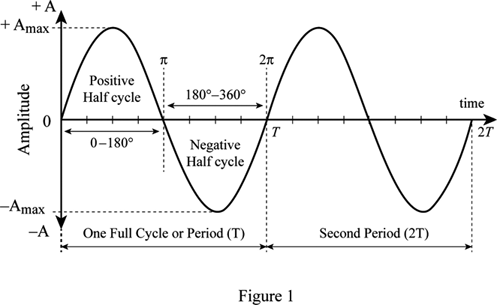
\includegraphics[width=0.45\textwidth]{sine}

 \caption[My first figure]%the text in [] will be displayed in the list of figures.  
  %If this is omitted, the full figure caption (follows in {}) will be displayed in the list of figures.
  {\label{fig:sine} My first figure, showing a plot of the sine function.}
 \vspace{0.5 in}
 \end{figure}

Fig.\ref{fig:sine} is produced by the following
\begin{verbatim}
 \begin{figure}
 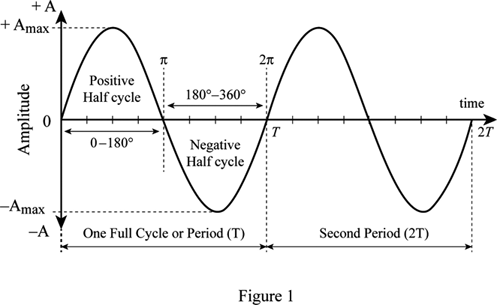
\includegraphics[width=0.45\textwidth]{sine}
 \caption[My first figure] 
  {\label{fig:sine} My first figure, showing a plot of the sine function.}
 \end{figure}
\end{verbatim}
The text \verb#[My first figure]# will be displayed in the list of figures.
If this is omitted, then the full figure caption (follows in \verb#{}#) 
will be displayed.  If you compile using \verb#latex#, then \verb#sine.eps# will be included.
If you compile using \verb#pdflatex#, then \verb#sine.pdf# will be used.  \verb#pdflatex#
also supports including \verb#.jpg# files if you prefer, but there can be artifacts when 
\verb#.jpg# files are rescaled, however one cannot always generate a PDF if an
image is ``borrowed'' (Fig.~\ref{fig:battery} uses jpegs).  
Note that you do \textbf{not} need to include a file extension 
for the figure - latex adds the appropriate extension automatically.  If you do
not want to place your figure in the same directory as the latex root document 
(in this case \verb#template.txt#), then you could instead use something like:
\begin{verbatim}
 \includegraphics[width=0.45\textwidth]{directory/figure}
\end{verbatim}

 \begin{figure}[h]
 \centering
\subfloat[Eating One Battery]{\label{one_battery}
 %The actual figure, part (a)
 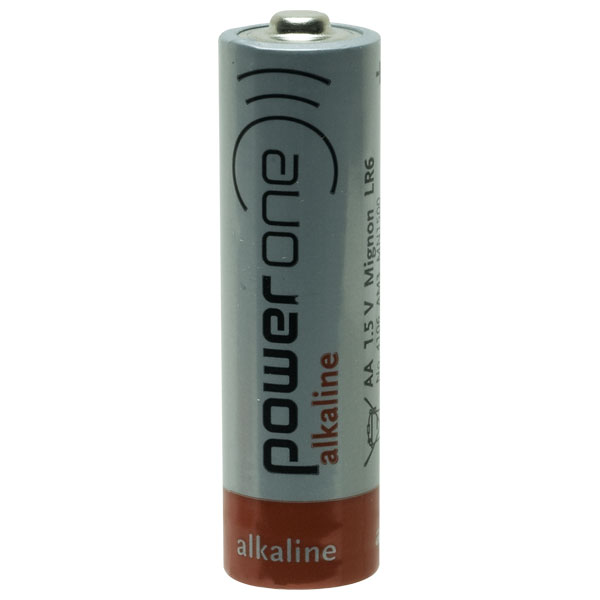
\includegraphics[width=0.45\textwidth]{one_battery}}
\hspace{0.5 in}
\subfloat[Eating Five Batteries]{\label{five_battery}
 %The actual figure, part (a)
 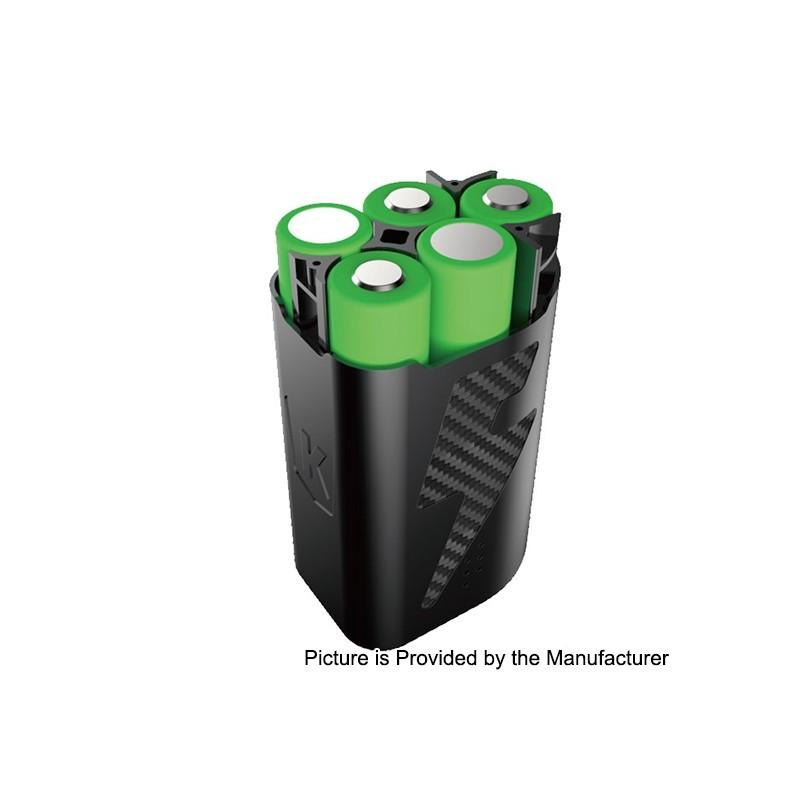
\includegraphics[width=0.3\textwidth]{five_battery}}


 \caption[Eating Batteries]%the text in [] will be displayed in the list of figures.  
  %If this is omitted, the full figure caption (follows in {}) will be displayed in the list of figures.
  {\label{fig:battery} A man eating batteries \cite{English}.  
  Reprinted with permission from Strong Bad.}
 \vspace{0.5 in}
 \end{figure}

Fig.\ref{fig:battery} is produced by the following
\begin{verbatim}
 \begin{figure}
\subfloat[Eating One Battery]{
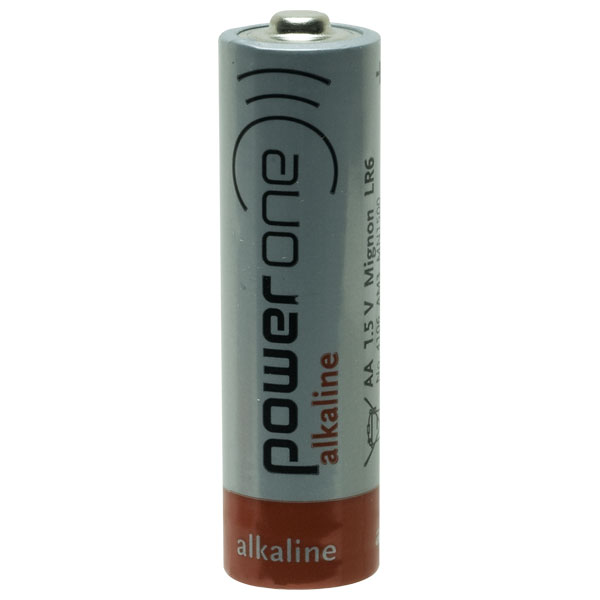
\includegraphics[width=0.45\textwidth]{one_battery}}
\subfloat[Eating Five Batteries]{
 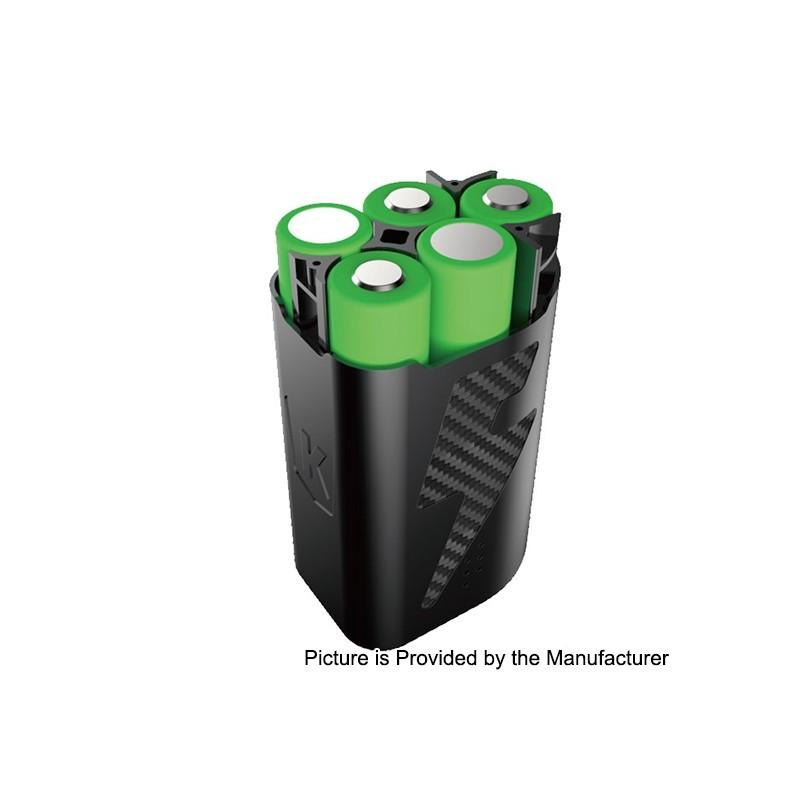
\includegraphics[width=0.3\textwidth]{five_battery}}
 \caption[Eating Batteries]
  {\label{fig:battery} A man eating batteries. Reprinted with permission from Strong Bad.}
 \end{figure}
\end{verbatim}
This figure is a reproduction of a figure from another ``work''.  
In this case the ``author'' gives explicit permission to reuse this figure,
but in most cases you will need to contact the journal to obtain permission to 
reproduce any part of an article, such as a figure.  
Journals are generally very nice about letting you reproduce figures 
for a thesis, and give permission very rapidly (sometime instantly online)
and don't charge anything.  However, if you do not obtain permission
you can have serious trouble after your thesis is published.
Note that you need to obtain permission to reuse figures
from any published paper, 
\textit{even if you are the author.} 

This figure also illustrates the use of subfigures via the subfig package, loaded by placing 
\verb#\usepackage{subfig}# in the preamble of \verb#template.txt#.  This allows you to include
each subfigure as an individual image, and have latex arrange and label them for you 
(including an optional name for each subfigure in \verb#[]#).  This also allows
you to individually reference Fig.~\ref{one_battery} and Fig.~\ref{five_battery}.
Note that many journals DO NOT support this, and require that each figure be a single
image, but this should be fine for a thesis.  


\section{This is a Section!}

\lipsum[2-4]
\subsection{This is a Subsection?}

\lipsum[5-10]

\subsubsection{This is a Subsubsection.}

\lipsum

\section{Another Section}

\lipsum[2-4]

\begin{table}
\begin{center}
\begin{tabular}{lll}
\hline
\\[3pt]
Alphabet Character & Vowel & Number \\[3pt]
\hline
\\[3pt]
A & Yes & 1 \\
B & No & 2 \\
C & No & 3 \\[3pt]
\hline
\end{tabular}
\label{tbl1}
\caption{My first Table}
\end{center}
\end{table}

\lipsum[4-6]
\begin{table}
\begin{center}
\begin{tabular}{lll}
\hline
\\[3pt]
Alphabet Character & Vowel & Number \\[3pt]
\hline
\\[3pt]
A & Yes & 1 \\
B & No & 2 \\
C & No & 3 \\[3pt]
\hline
\end{tabular}
\label{tbl2}
\caption{My second Table}
\end{center}
\end{table}

\lipsum[1-12]
\begin{equation}
\partial_\mu F^{\mu\nu} = J^\nu
\end{equation}
Lorem ipsum your face. Lorem ipsum your face. 

\lipsum[1]A footnote\footnote{Another foot.}.\lipsum[2-5]
\begin{equation}
E = \gamma mc^2
\end{equation}
Lorem ipsum your face. Lorem ipsum your face. 

\lipsum[2-5]

\chapter{The Plot Thickens and the Page Numbering Progresses, and Boy is This Title Really, Really, Really Long}

\lipsum[1] A long footnote\footnote{Footnote after Chapter. Did I
  reset? What is my line spacing... I should make this a really long
  footnote to find out.  Here we go. \lipsum[1] This ought to be long
  enough.}.
\begin{table}
\begin{center}
\begin{tabular}{lll}
\hline
\\[3pt]
Alphabet Character & Vowel & Number \\[3pt]
\hline
\\[3pt]
A & Yes & 1 \\
B & No & 2 \\
C & No & 3 \\[3pt]
\hline
\end{tabular}
\label{tbl3}
\caption{Another Table}
\end{center}
\end{table}

\lipsum
\section{doo-da}

\lipsum[2-6]
\section{It's a Section, Bitch}

\lipsum

\chapter{What a Chapter!}

\lipsum[2-10]

\section{Whose Section is this Anyways?}

\lipsum
\section{I think I am Funny, But I am Not}

\lipsum[1-3]
\subsection{Running Out of Headings Here}

Lorem ipsum~\cite{bib3}.  Lorem ipsum dolor sit amet. 
\lipsum[1]

\lipsum

\chapter{Let It End}

\lipsum[1]
\section{Please?}

\lipsum



\backmatter
% We use BIBTeX for the bibliography---you don't have to
\bibliographystyle{unsrt} % use your favorite BIBTeX style
% \nocite{*} % To display all refs, even uncited refs (useful when editting)
\bibliography{templatebib}

% If for some reason you are anti-BIBTeX, then you would use the
% following instead of the above:
%\begin{thebibliography}{99}
% ...
%\end{thebibliography}


% Note: GS 2010 requires bibliography/references _before_ the appendix
% if you believe their guidelines; however, conversations with GS
% staff suggests _they don't care_. Go figure. So do what you like.

\appendix
\chapter{My Appendix needs to be removed...}


A citation~\cite{bib2}. \lipsum[1]

\section{Sections in an Appendix, What is the World Coming to?}

Another citation~\cite{bib1}.  \lipsum[1]
\begin{equation}
\frac{1}{\sqrt{2\pi \sigma^2}}e^{-\frac{1}{2}(\frac{x-\mu}{\sigma})^2}
\end{equation}
\lipsum[1]

\subsection{Subsections, Too!}

\lipsum[2-5]
\begin{equation}
e^{i\pi} + 1 = 0
\end{equation}
\lipsum[1-3]

\chapter{I don't feel so good}

\lipsum


\end{document}
